\documentclass[12pt,a4paper]{article}
\usepackage[latin1]{inputenc}
\usepackage{amsmath}
\usepackage{amsfonts}
\usepackage{amssymb}
\usepackage{graphicx}
\usepackage[parfill]{parskip}
\usepackage{caption}
\usepackage{subcaption}

\author{Jeremy Scheurer}
\title{Solutions to exercises of "Reinforcement Learning: An Introduction" (Sutton and Barto)}
\date{Created in February 2018}


\begin{document}

\maketitle
\tableofcontents
\newpage
	
\section{Chapter 1: The reinforcement learning problem}
\subsection{Self-Play }
\textit{Suppose, instead of playing against a random opponent, the reinforcement learning algorithm 		described above played against itself, with both sides learning. What do you think would happen in this case? Would it learn a different policy for selecting moves?}\\

Well for one thing we cannot let the learning rate go to zero, because our opponent is constantly changing(learning) and thus we need to adopt aswell. Before we assumed that our opponent plays imperfectly, if this is still the case for ourself, then exploiting a certain weakness might only work once, because the opponent will learn about it. I guess it would still learn the same policies but as both sides improve in the end they will both have found out the best possible moves and thus nobody will ever win.

\subsection{Symmetries}
\textit{Many tic-tac-toe positions appear different but are really the same because of symmetries. How might we amend the learning process described above to take advantage of this? In what ways would this change improve the learning process? Now think again. Suppose the opponent did not take advantage of symmetries. In that case, should we? Is it true, then, that symmetrically equivalent positions should necessarily have the same value?} \\ 

We could have not a different value estimation for each possible state the board can be in, but for groups of states. These groups of states each contain states thate are symmetric to each other. By doing this we would have less states in total which would mean we have to explore less to visit each state for at least one time. That means we can have faster convergence to an optimal solution. \\
Well the problem is that if our oponent does not take advantage of symmetries he could be playing very differently in several states that are symmetric. He could always be playing perfectly in one state and imperfectly in the other. We would then not be able to capture this difference, because both states are just one state in our model. So it is not necessarily true that symmetrically equivalent positions should have the same value.

\subsection{Greedy Play }
\textit{Suppose the reinforcement learning player was greedy, that is, it always played the move that brought it to the position that it rated the best. Might it learn to play better, or worse, than a nongreedy player? What problems might occur?}\\ 

For this question I will assume that we are not using the UCB algorithm or similar algorithms where taking the greedy choice also includes sometimes exploring states. Thus always making the greedy choice obviously neglects exploring other states. So if you are very lucky you might just make all the optimal actions by always choosing the greedy choice. But this is very unlikely, most probably you will never be able to reach the optimal solution. If we compare this with an intelligent non-greedy algorithm which will explore different actions, this greedy-algorithm clearly underperforms. 

\subsection{Learning from Exploration}
\textit{Suppose learning updates occurred after all moves, including exploratory moves. If the step-size parameter is appropriately reduced over time (but not the tendency to explore), then the state values would converge to a set of probabilities. What are the two sets of probabilities computed when we do, and when we do not, learn from exploratory moves? Assuming that we do continue to make exploratory moves, which set of probabilities might be better to learn? Which would result in more wins?} \\

The problem is that with exploratory actions anything can happen. So if I have a state which is actually the best state to win and then take an exploratory action which turns out to lead to a very bad state, I will then update the previous state into the direction of the new(bad) state. Depending on the learning rate this can lead to updating the previous state more strongly or not. But obviously this could lead to a scenario where the previous state, which was very good, now is considered as a bad state(with obviously no good reason for that, because we were only exploring). So in the first case, where we do not update after exploring, the probabilities we try to approximate are the ones that lead to the most wins. So we try to learn how our opponent plays and exploit its deficiencies. In the second case basically anyhting could happen and the probabilities cannot be interpreted with sense. 

\subsection{Other improvements}
\textit{Can you think of other ways to improve the reinforcement learning player? Can you think of any better way to solve the tic-tac- toe problem as posed?} \\

One important thing was already mentioned, namely to keep the learning-rate from becoming zero. Only then can we always adapt to a changing opponent. One could also play against itself to keep improving and to learn different opposing behaviour. One important thing we also have to introduce is the uncertainty about our state-values. We should also explore actions we are uncertain about, more often(see later UCB algorithm).

\section{Multi-armed Bandits} 
\subsection{Longterm epsilon greedy}
\textit{In the comparison shown in Figure 2.2, which method will perform best in the long run in terms of cumulative reward and cumulative probability of selecting the best action? How much better will it be? Express your answer quantitatively.} \\

The greedy algorithm with epsilon = 0.01 will perform better than the one with epsilon 0.1 in the long run. The second algorithm will be able to find the best action more quickly but never takes it more than 0.91 \% of the time. In contrast the first algorithm will take longer to find the optimal action, but will eventually find it. And once it does, it will take it about 0.99 \% of the time. So it will be about 8-9 \% better than the second option. 

\subsection{Step-size parameters}
\textit{If the step-size parameters $\alpha_n$, are not constant, then the estimate $Q_n$ is a weighted average of previously received rewards with a weighting different from that given by (2.6). What is the weighting on each prior reward for the general case, analogous to (2.6), in terms of the sequence of step-size parameters?} \\ 
The alpha's are not constant but can be any value such as $ \alpha = \frac{1}{n}$. Thus we get the following formula from 2.6 by replacing the alpha's: \\
$ (1-\alpha_1)^nQ_1 + \sum_{i=1}^{n} \alpha_i(1-\alpha_i)^{n-i}R_i $

\subsection{Optimistic vs Realistic greedy}
\textit{The results shown in Figure 2.3 should be quite reliable because they are averages over 2000 individual, randomly chosen 10-armed bandit tasks. Why, then, are there oscillations and spikes in the early part of the curve for the optimistic method? In other words, what might make this method perform particularly better or worse, on average, on particular early steps?}

Because compared to the realistic greedy method, in the first n steps each of the n arms is pulled exactly once. That means that after exploring each arm, for one round at least we are very likely to choose the optimal action. This  implies that we will definitely have a sharp spike in the optimal action vs steps plot. For comparison, the realistic greedy method explores much less and has much less chance of finding out about the optimal action in the early rounds. 

\subsection{Programming: }
\textit{Design and conduct an experiment to demonstrate the difficulties that sample-average methods have for nonstationary problems. Use a modified version of the 10-armed testbed in which all the q*(a) start out equal and then take independent random walks. Prepare plots like Figure 2.2 for an action-value method using sample averages, incrementally computed by $\alpha = 1$ , and another n action-value method using a constant step-size parameter, $\alpha= 0.1$. Use $\epsilon$ = 0.1 and, if necessary, runs longer than 1000 steps.} \\ 

Remember the update rule of the iterative sample-average method: New estimate = Old Estimate + stepsize * [old estimate - target]. As seen in the book, the problem about non-constant step-sizes like $\frac{1}{n}$ is that if we have a non-stationary problem, they cannot adapt anymore after a certain time, because we are not updating the old estimate enough anymore(because the stepsize goes to zero). \\ 
By running different experiments with 1000 steps and a 1000 repetitions we got the following: \\
\begin{figure}[h]
\begin{subfigure}{.5\textwidth}
 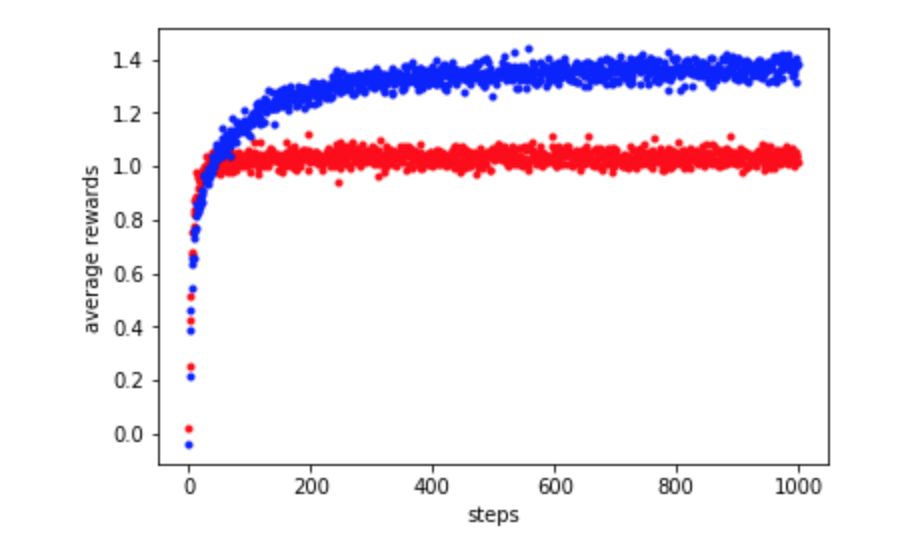
\includegraphics[width=1\textwidth, height = 150px]{images/epsilon_greedy_comparison.png}
 \caption{Epsilon greedy algorithm on a stationary problem. \\Blue: $\epsilon = 0.1$, Red: $\epsilon = 0.0$}
\end{subfigure}
\begin{subfigure}{.5\textwidth}
 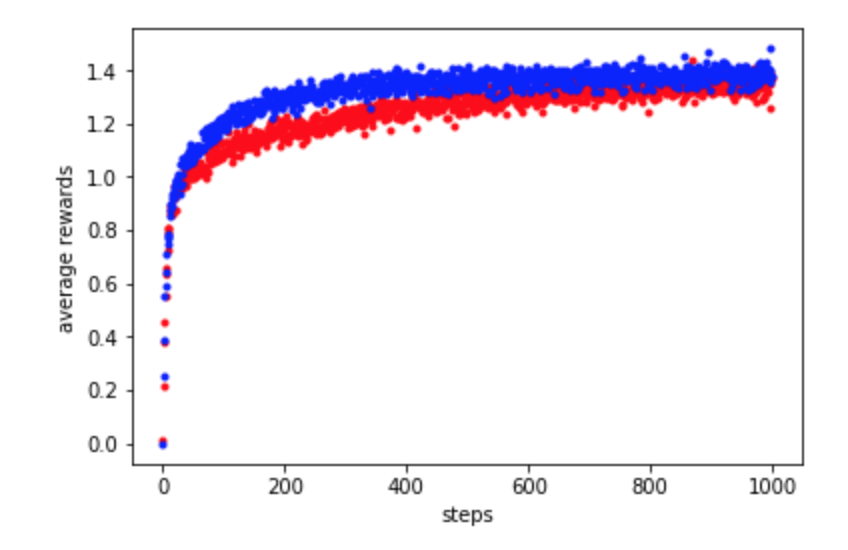
\includegraphics[width=1\textwidth, height = 150px]{images/stepsize_comparison_stationary.png}
 \caption{Epsilon greedy algorithm with $\epsilon = 0.1$ on a stationary problem.\\ Blue: stepsize = $\frac{1}{n}$, Red: stepsie = 0.1}
 \end{subfigure}

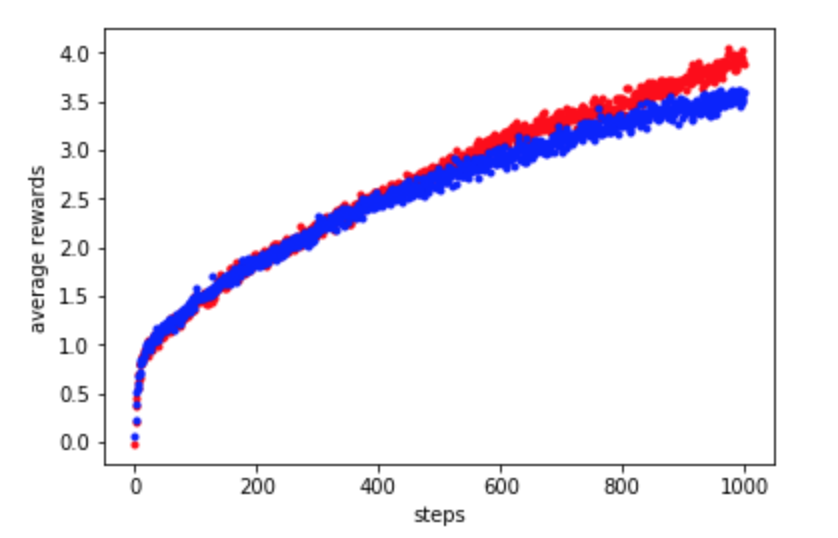
\includegraphics[width=0.7\textwidth, height = 150px]{images/stepsize_comparison_non_stationary.png}
\centering
\caption{Epsilon greedy algorithm with $epsilon = 0.1$ on a non-stationary problem. \\ Blue: stepsize = $\frac{1}{n}$, Red: stepsie = 0.1}
\end{figure}

\begin{figure}
	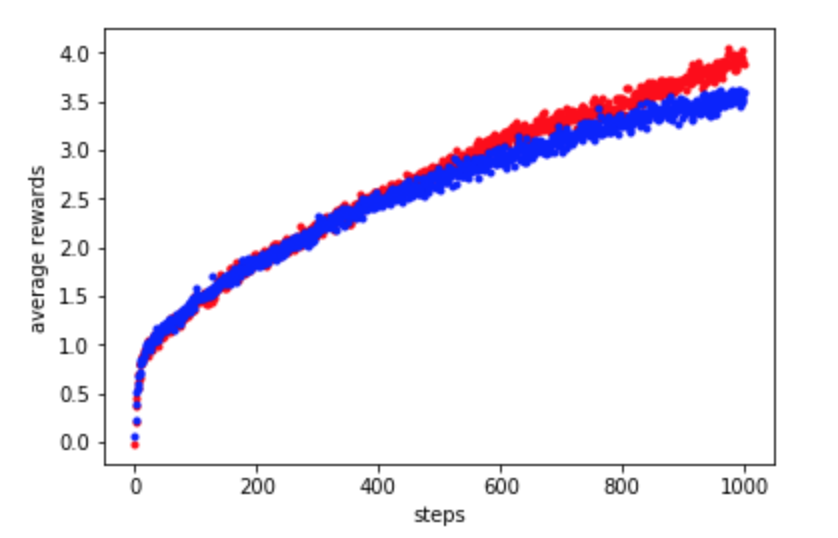
\includegraphics[width=0.7\textwidth, height = 130px]{images/stepsize_comparison_non_stationary.png}
	\caption{Epsilon greedy algorithm with $epsilon = 0.1$ on a non-stationary problem. \\ Blue: stepsize = $\frac{1}{n}$, Red: stepsie = 0.1}
\end{figure}
 
For code solutions see Coding/Chapter02/Exercise2.4


\subsection{Spike in UCB plot}
\textit{In Figure 2.4 the UCB algorithm shows a distinct spike in performance on the 11th step. Why is this? Note that for your answer to be fully satisfactory it must explain both why the reward increases on the 11th step and why it decreases on the subsequent steps. Hint: if c = 1, then the spike is much less prominent.} \\ 

I am not so sure about this answer, but I think it is a similar reasoning as my answer in 2.3. If we have a larger c, we explore more. We see that the initial average rewards are very small, thus increasing t will make the confidence bound of the not yet selected arms definitelly larger than the already explored arms. This leads to a probable scenario where in the first 10 steps we explore each arm exactly once. So from the eleventh step on we will not consider "bad" arms for a longer period(until t is large enough) and will choose one of the better arms with a high likelihood. 

Note to myself: The fishy thing about this idea is that after one round, our confidence about which arm is good or bad is very low. So there is a high likelihood that a "bad" arm yields a good reward and vice versa. This contradicts the argument form above. 
\end{document}


